\subsection{Front}
\begin{figure}[h!]
 \centering
 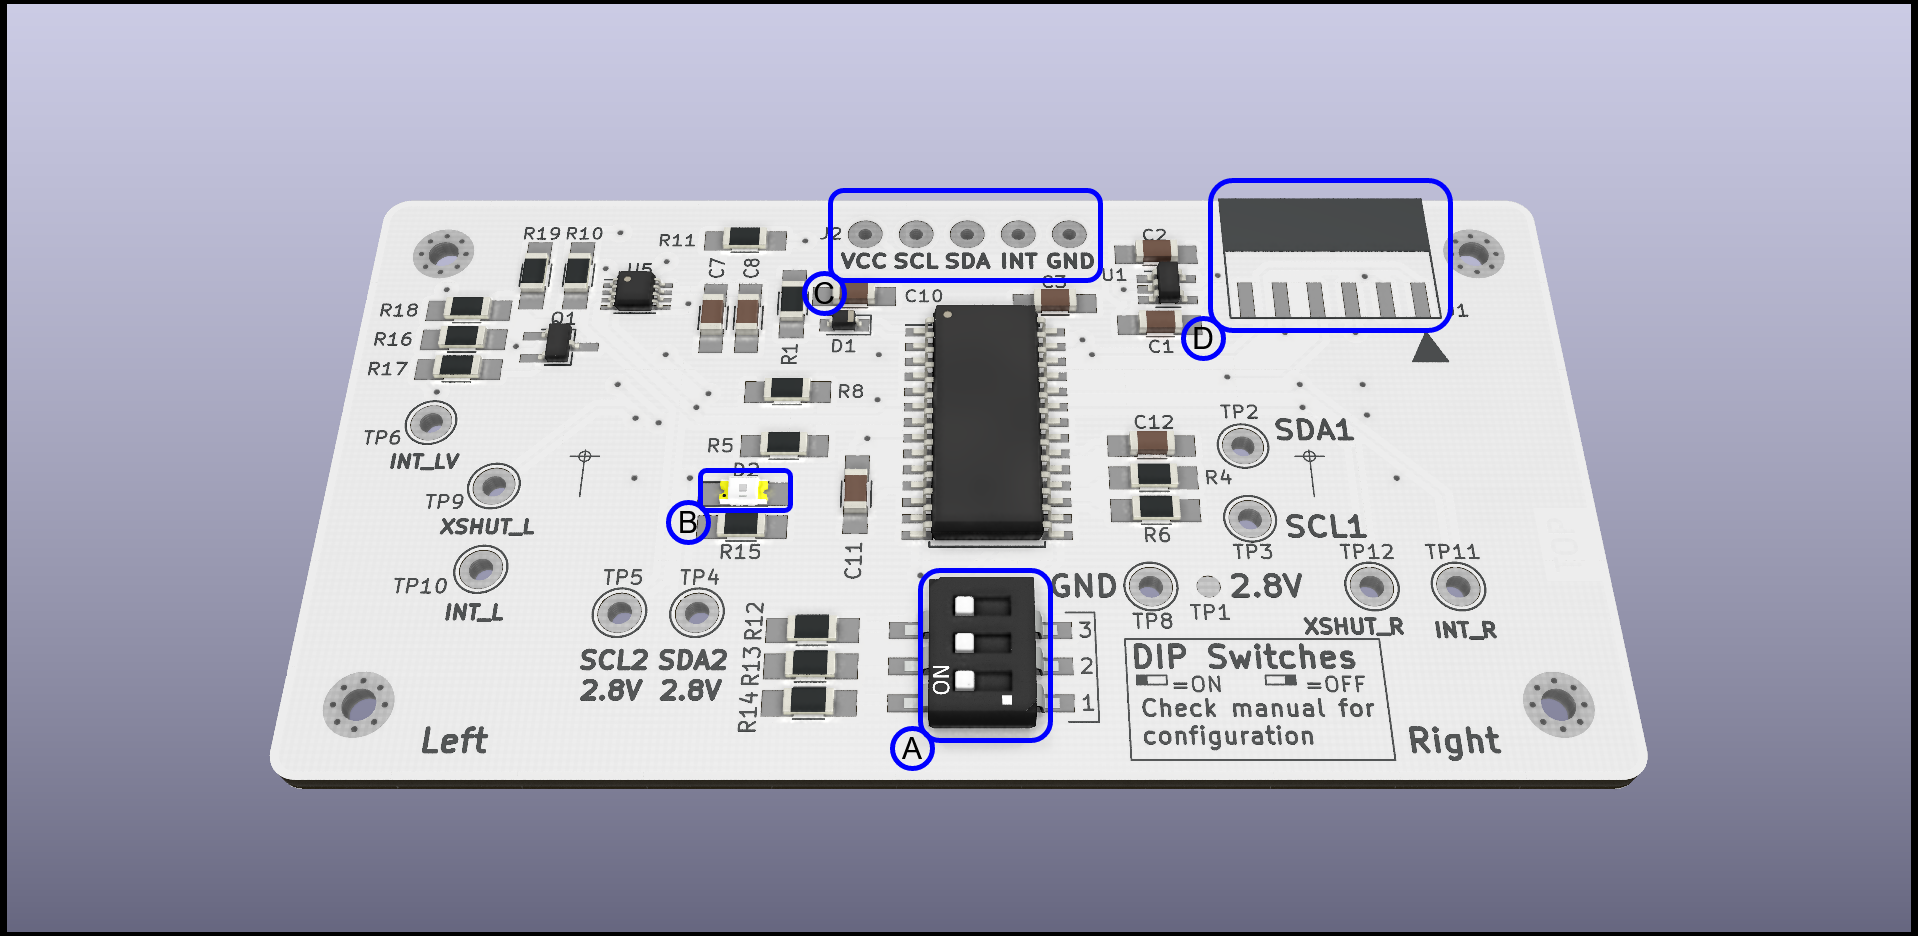
\includegraphics[width=0.75\textwidth]{../img/V1.1/annotated-layout-front.png}
 \caption{Annotated picture of the front of the sensor}
\end{figure}
\begin{itemize}
 \item[A] Boot configuration DIP Switches.
 \item[B] LED indicator
 \item[C] Main connector (Power, \iic, Interrupts)
 \item[D] ICSP connector to program the PIC controller
\end{itemize}
\textit{\textbf{Note: }On PCB V1.0 the \texttt{XSHUT} and  \texttt{INT} test points labels have been swapped for the right and left sensors.}

\subsection{Back}
\begin{figure}[H]
 \centering
 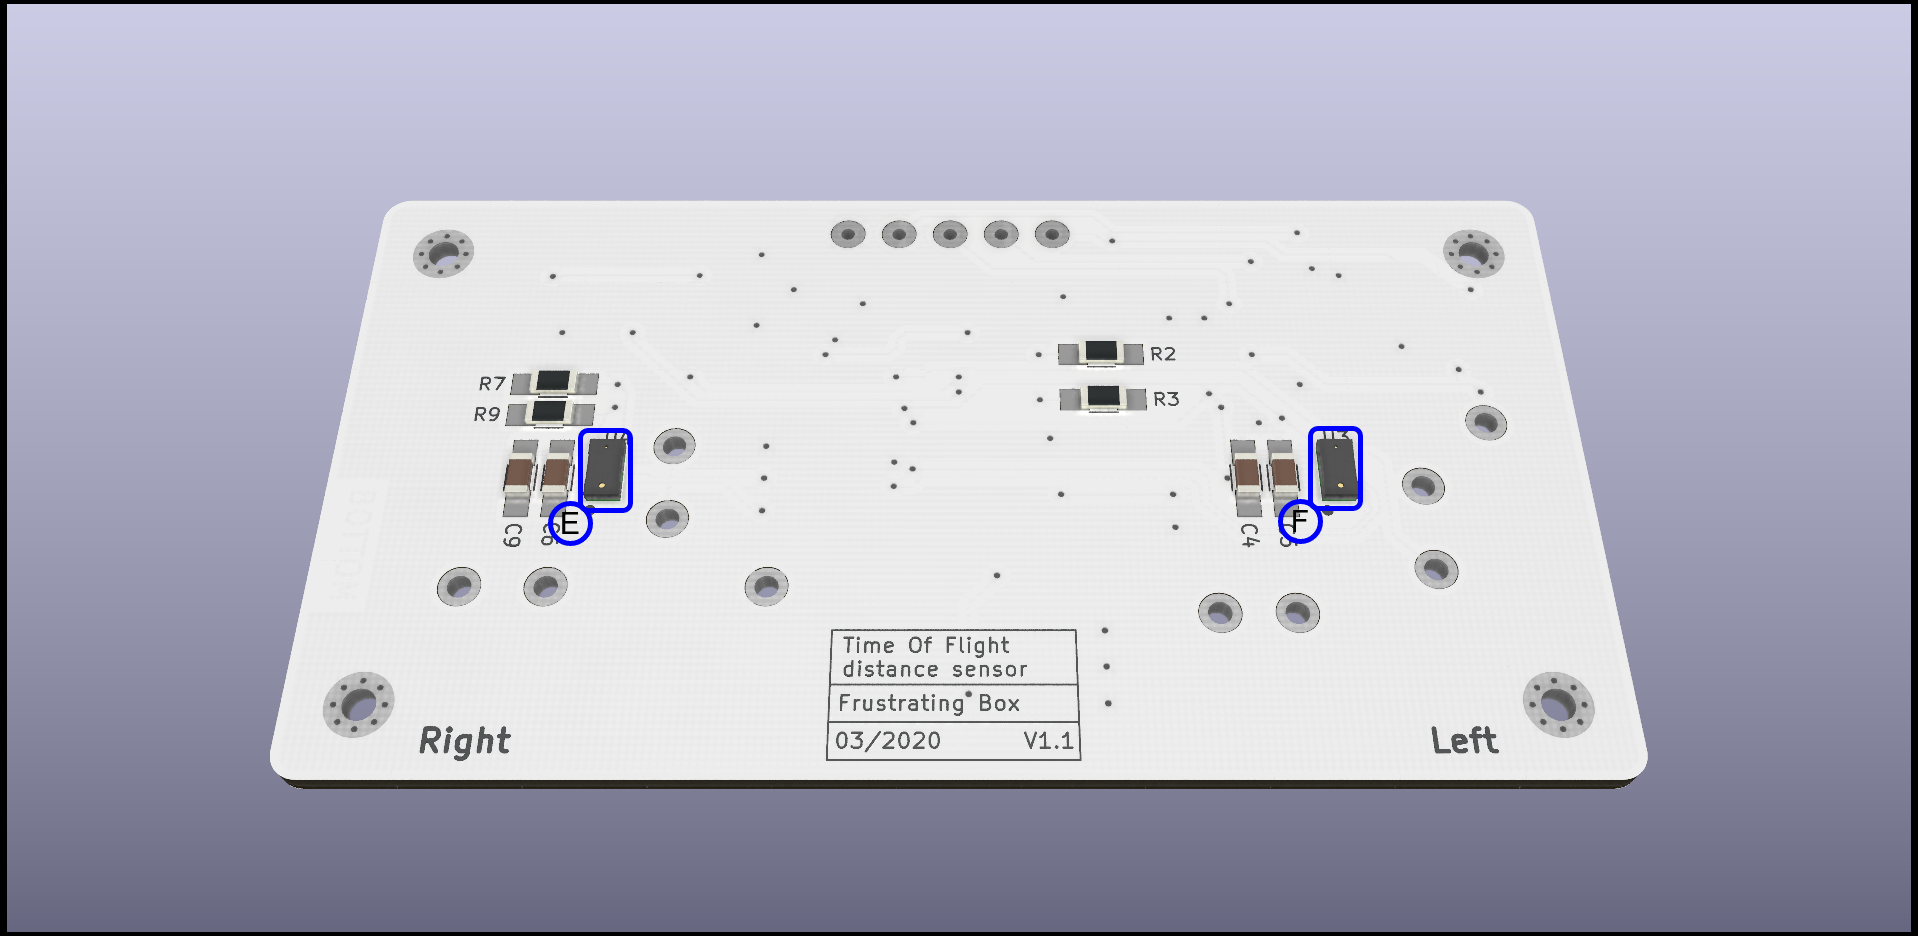
\includegraphics[width=0.75\textwidth]{../img/V1.1/annotated-layout-back.png}
 \caption{Annotated picture of the back of the sensor}
\end{figure}
\begin{itemize}
 \item[E] Right sensor
 \item[F] Left sensor
\end{itemize}